% ================================ 3. DATA ================================
\section{Data}\label{sec:data}

\subsection{The order file}

The dataset is the order file released for the 2017 Mobike Algorithm Challenge
\cite{mobike}.

The dataset contains 3,214,096 order records. Each record has an order identifier, a
user identifier, a bicycle identifier, a bicycle type, a start timestamp and two
seven-character geohashes that encode the start and end positions. Decoding follows
the standard base-32 latitude/longitude interleaving \cite{niemeyer2008}: each
character contributes five bits, alternately to longitude and latitude, so that a
seven-character string resolves a rectangle of roughly $153\times153$ m. The decoded
coordinates agree with the operator's own city, and 99.6\% of the records begin with
the geohash prefix \texttt{wx4}, which covers Beijing.

We remove 786 records whose decoded start lies outside the metropolitan bounding box
($39.4$--$40.4^\circ$N, $115.8$--$117.0^\circ$E); these are GPS or decoding faults as
far away as $20^\circ$N. After the filter 3,213,310 orders remain, placed by 349,241
users on 484,754 distinct bicycles.

\subsection{Coverage, and why the analysis uses seven days}

\figref{fig:data}a shows the daily volume. Three features matter.

The volume is stable at 225,000--322,000 orders per day from 10 to 19 May, with the
weekend dip one expects. \textbf{17 May is entirely absent} --- not sparse, absent ---
so no interpolation is possible and we treat the day as missing.

From 20 May onward the volume falls to 120,000--210,000 and stays there. The drop is
too abrupt to be behavioural, and the hourly profile of those days is
indistinguishable from the earlier ones; it is a truncation of the operator's sample,
not a change in the city. We therefore restrict all estimation to the ten days
10--19 May, and within them to the seven weekdays that are fully covered, which we
call \emph{typical days}. Weekends are used only where the text says so.

\begin{figure}[htbp]
\centering
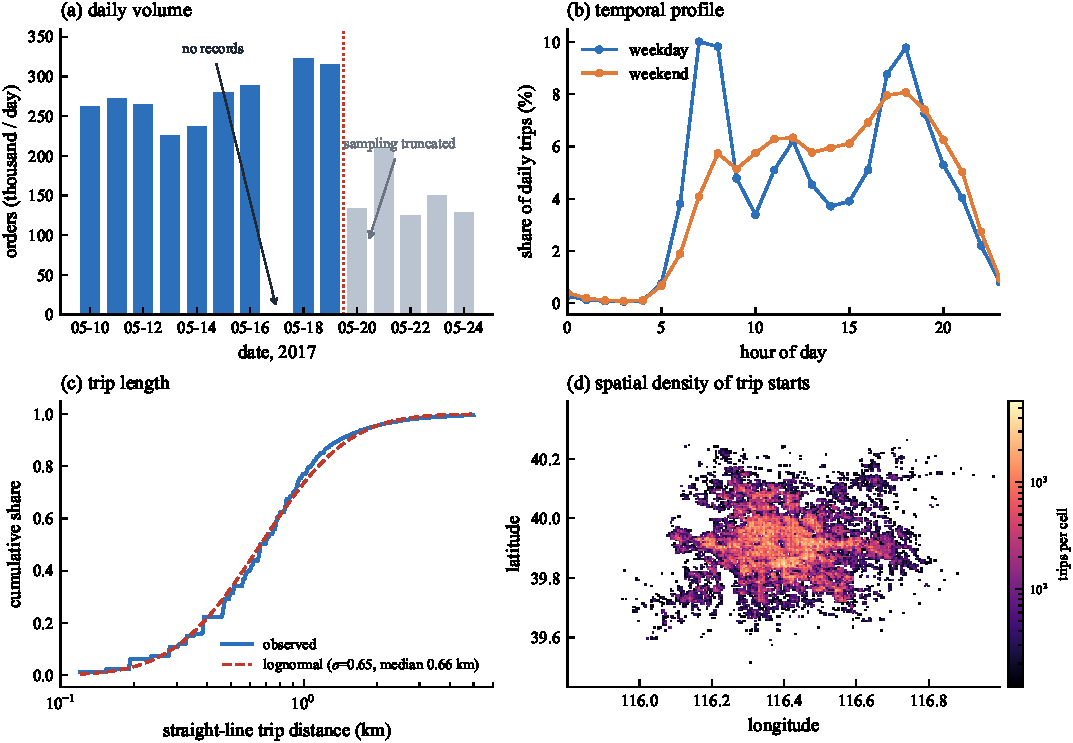
\includegraphics[width=0.9\linewidth]{../figs/fig1_data.pdf}
\caption[The dataset]{The dataset. (a) Daily order volume; 17 May has no records and the sample is
truncated from 20 May. (b) Hourly profile, weekdays against weekends. (c) Empirical
distribution of straight-line trip distance with a fitted lognormal. (d) Spatial
density of trip starts, logarithmic colour scale.}
\label{fig:data}
\end{figure}

\subsection{The sampling rate}

The file is a sample of the operator's orders, not a census. If each order is retained
independently with probability $p$, then every count must be divided by $p$, and the
number of distinct bicycle identifiers understates the fleet. We estimate $p$ from
the bicycles themselves.

For a given bicycle, consider two consecutive orders that both appear in the file.
They are adjacent in the bicycle's true history exactly when no order between them was
dropped, which for independent retention happens with probability $p$. Adjacency is
observable: if the two orders are adjacent, the bicycle was not moved in between, so
the second order must start in the same 153 m geohash cell in which the first ended.
Conversely, a mismatch proves that at least one order is missing. Across all bicycles
with two or more orders, \textbf{12.8\% of consecutive pairs satisfy the
end-equals-next-start test}.

Two biases act in opposite directions and both are small. A bicycle re-parked within
the same 153 m cell after an unobserved trip creates a false match, which makes 12.8\%
an overestimate of the match rate and hence a \emph{lower} bound on $p$; a bicycle
locked a few metres away but across a cell boundary creates a false mismatch. We adopt
$p=0.128$ and treat it as an order-of-magnitude estimate. Section~\ref{sec:sens}
shows that this uncertainty does not propagate into the fleet estimate at all.

\subsection{Fleet size}

The file contains no inventory, so the fleet must be inferred from the pattern of use.
Model each bicycle as being ridden a random number of times per day with mean $\mu$,
Poisson distributed across bicycles and independent across days. A bicycle appears in
the data at least once with probability $1-e^{-\mu}$. With $T$ orders and $D$ distinct
bicycles observed on a day,
\begin{equation}
\frac{T}{D} \;=\; \frac{\mu}{1-e^{-\mu}},
\label{eq:fleet}
\end{equation}
which is strictly increasing in $\mu$ and therefore invertible. For the reference
weekday $T/D=1.478$, giving $\mu=0.840$ and
\begin{equation}
\hat F \;=\; \frac{T}{\mu} \;=\; 343{,}638 \ \text{bicycles}.
\end{equation}

The estimate is invariant to the sampling rate, which is worth showing because it is
the reason the unidentified $p$ does no damage. Under retention probability $p$ the
observed quantities are $T_p=pT$ and $D_p=F(1-e^{-p\mu})$, so
$T_p/D_p=p\mu/(1-e^{-p\mu})$. Inverting \eqnref{eq:fleet} on the observed ratio
returns $p\mu$, and $\hat F=T_p/(p\mu)=T/\mu$. Resampling the orders at rates from 5\%
to 50\% reproduces $\hat F$ within 4\% (Section~\ref{sec:sens}), which confirms the
algebra numerically.

At 343,638 bicycles and $2.14\times10^6$ rides per day, each bicycle is ridden
\textbf{6.2 times per day}. For comparison, a private car is driven three to four times
per day; the fleet is worked hard in the aggregate and idle in the particular, which
is the tension the rest of the paper quantifies.

\subsection{Spatial units}

Two partitions are used, at different resolutions and for different purposes.

\textbf{Cells.} A grid of $0.005^\circ$ (about $555\times426$ m) is laid over the
city. Keeping only cells with at least 50 sampled trips leaves \textbf{5,263 cells},
which contain 95.8\% of the typical-day trips. Cells are the unit at which a rider can
reasonably be asked to change destination (a few hundred metres), so they are used for
the incentive model (Q3) and the parking model (Q4).

\textbf{Zones.} Fifty zones are formed by $k$-means on the cell centroids weighted by
trip volume, and each cell is assigned to its nearest centroid. Zones hold between
604 and 12,119 trips per day and are roughly 4 km across, which is the scale at which a
truck moves bicycles. They are used for rebalancing (Q2).

\tabref{tab:data} collects the descriptive statistics.

\begin{table}[htbp]
\centering
\caption[Data summary after cleaning]{Data summary after cleaning. Distances are straight-line between decoded
endpoints.}
\label{tab:data}
\small
\begin{tabular}{@{}lrl@{}}
\toprule
\textbf{Quantity} & \textbf{Value} & \textbf{Note} \\
\midrule
Order records & 3,213,310 & after bounding-box filter (786 removed) \\
Users & 349,241 & \\
Bicycles & 484,754 & distinct identifiers over 14 days \\
Dates present & 14 & 17 May absent \\
Typical days used & 7 & fully covered weekdays \\
Trips per typical day (sample) & 274,357 & \\
Trips per typical day (scaled) & $2.14\times10^6$ & $p=0.128$ \\
Median trip distance & 0.70 km & lognormal $\sigma=0.65$ \\
90th percentile distance & 1.41 km & \\
Study cells & 5,263 & $\geq50$ trips, $0.005^\circ$ grid \\
Traffic zones & 50 & weighted $k$-means \\
Fleet estimate & 343,638 & Eq.~\eqref{eq:fleet} \\
Rides per bicycle per day & 6.2 & scaled trips / fleet \\
\bottomrule
\end{tabular}
\end{table}

Two remarks on the distance distribution (\figref{fig:data}c). It is close to
lognormal, with an empirical median of 0.70 km and a 90th percentile of 1.41 km, but
the fit is not exact: the lognormal drawn in the figure has $\sigma=0.65$ and a median
of 0.66 km, and the 0.04 km by which it undershoots the empirical median is the
compressed lower tail, because trips shorter than about 150 m cannot be distinguished
from zero at the geohash resolution. This is a measurement floor, not a behavioural
feature, and the gravity model is estimated on the distances that are resolved.
